\subsubsection{An\'alise Explorat\'oria dos dados (EDA)}

A partir de \ref{etp:1} é realizado o EDA para o processamento de dados obtidos até agora, com EDA será respondido. De acordo com a \citeonline{Yu2016} Na era dos grandes dados, coletamos volumes de dados em massa caóticos, não estruturados e multimídia através de vários canais. Como descobrir as regras, modelos analíticos e hipóteses destes dados se tornou o novo desafio. A análise exploratória de dados foi promovida por John Tukey para encorajar os estatísticos a explorar os dados e possivelmente formular hipóteses que poderiam levar a uma maior coleta de dados e experimentos. Em contraste com a análise inicial de dados, a análise exploratória de dados (EDA) é uma abordagem para analisar conjuntos de dados para resumir suas principais características, muitas vezes com métodos visuais. Muitas técnicas de EDA têm sido adotadas em grandes análises de dados.

Olhando o \ref{q1} relacionando a demanda com a variável prevista e a pressão para a variável PT01 na Figura \ref{fig:person} pode-se ver que ambas estão trabalhando igualmente, quase uma correlação perfeita de $r=1$, então para esta pergunta basta olhar para a correlação Pearson na Figura \ref{fig:person}. 

Para \ref{q2} uma tabela é feita para responder melhor a esta pergunta


\begin{table}[H]
	\centering
	\caption{Descrição estatística dos dados com o filtro aplicado das 18h às 21h}\label{tb:est}
	\begin{tabular}{@{}cccccccccc@{}}
		\toprule
		\textbf{18 a 21h}  & \textbf{B1} & \textbf{B2} & \textbf{B3} & \textbf{LT01} & \textbf{FT01} & \textbf{FT02} & \textbf{FT03} & \textbf{PT01} & \textbf{PT02} \\ \midrule
		\textbf{Contagem} & 366         & 366         & 366         & 366           & 366           & 366           & 366           & 366           & 366           \\
		\textbf{Média}    & 43,87       & 22,26       & 8,70        & 3,34          & 164,83        & 133,08        & 102,01        & 4,23          & 17,29         \\
		\textbf{STD}      & 23,22       & 18,47       & 17,81       & 0,69          & 114,60        & 67,99         & 47,55         & 0,81          & 8,59          \\
		\textbf{Min}      & 0           & 0           & 0           & 0,99          & 0,07          & 0             & 0             & 1,88          & 0             \\
		\textbf{25\%}     & 37,93       & 0           & 0           & 2,87          & 64,31         & 131,06        & 107,92        & 3,69          & 16,77         \\
		\textbf{50\%}     & 57,99       & 30,92       & 0           & 3,41          & 201,37        & 146,17        & 121,40        & 4,22          & 22,46         \\
		\textbf{75\%}     & 57,99       & 37,25       & 0           & 3,86          & 268,61        & 158,71        & 127,07        & 4,85          & 22,52         \\
		\textbf{Max}      & 59,99       & 57,33       & 53,74       & 4,40          & 379,20        & 285,56        & 170,56        & 5,66          & 24,23         \\ \bottomrule
	\end{tabular}
	
	Fonte: Elaboração própria a partir de dados da SANEPAR (2018 a 2020)
\end{table}

Na tabela \ref{tb:est} o desvio padrão é dado pela sigla STD que vem do inglês \textit{standard deviation} também observando para responder ao \ref{q2} assim como toda empresa de tratamento de água é feito um acionamento automático chamado trava de segurança para que o tanque não chegue a zero e falte água em todos os lugares adjacentes que é abastecida por esta água, este mínimo que o tanque pode alcançar é $1.459 m^3\Longleftrightarrow 1459 $ litros e as bombas serão ativadas em sua potência máxima para evitar a ativação das bombas o nível do tanque tem que estar na faixa de $[3.843,4.256]\ m^3$ bomba 1 ainda estaria funcionando para completar o nível. Em casos de pico, o mais ideal, mas não o mais rentável, é outro tanque de reserva nesses momentos e instalar uma tubulação para conectar uma à outra. Durante o dia, ambos estariam abastecendo e à noite, por gravidade, ficariam com o mesmo nível até que o consumo atingisse um nível para acionar as bombas.  



%\begin{figure}[H]
%	\centering
%	\caption{Solução para o acionamento das bombas}
%	\label{fig:esquema}
%	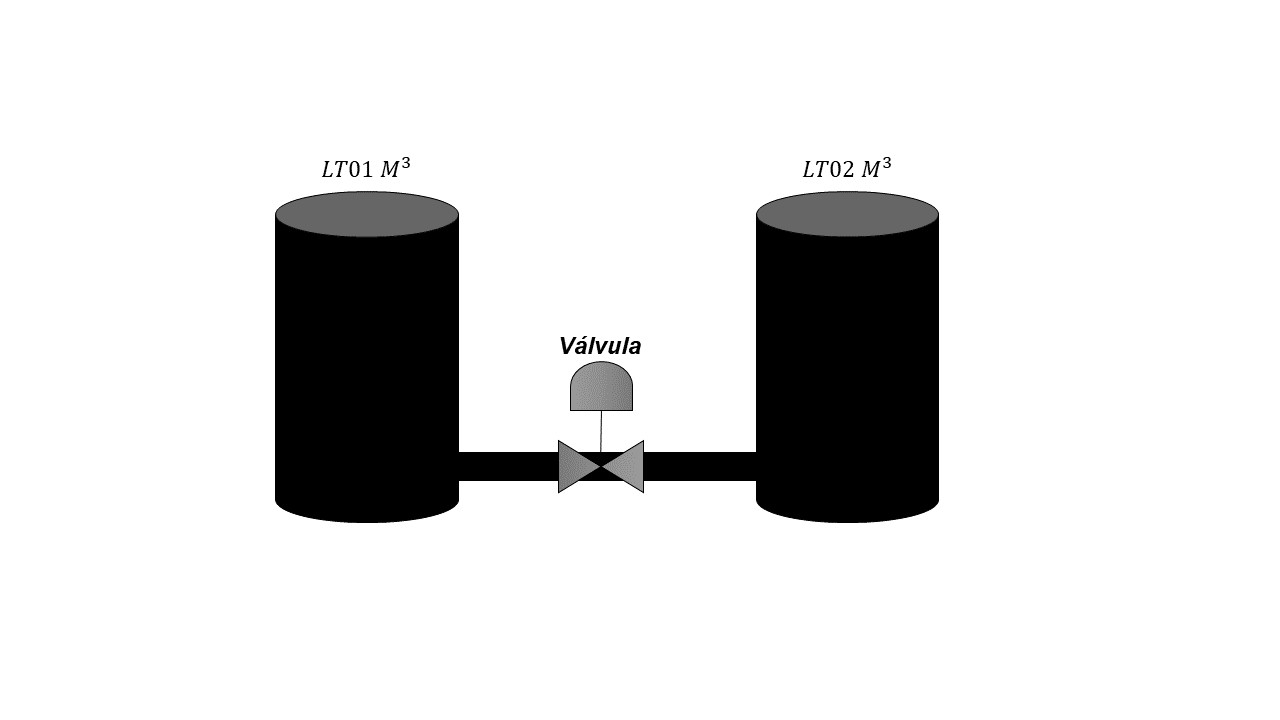
\includegraphics[width=1\linewidth]{Resultados/Figuras/esquema}
%	Fonte: Elaboração própria 
%\end{figure}
%
%Na Figura \ref{fig:esquema} um esquema prático para evitar a escassez de água e o consumo em horários de pico. Este é um esquema muito simples de como a hora do dia pode ser melhorada para o armazenamento de água.

Na \ref{q3} o tanque tem como máximo nos dados $4,256 m^3$ de dano em litros $4256$L para atender esta demanda e manter o tanque quase cheio ou sempre cheio o fluxo de entrada tem que estar entre $[238,302] \ m^3/h$ fluxo de gravidade tem que estar entre $[126,182] \ m^3/h$ fluxo de retorno entre $[110,144] \ m^3/h$ pressão de sucção entre $[1.92,4.24] mca$, pressão de retorno entre $[21,24] \ mca$.

Para \ref{q4}, o ponto de equilíbrio para não iniciar as bombas seria o fluxo FT01 $211 m^3/h$ FT02 $114 m^3/h$ FT03 $100m^3/h$ e o nível do tanque a $3,545 m^3$.

Ao \ref{q5}\ref{q5:a} o tanque deve estar a um nível de $4,00 m^3$ para que não precise funcionar com bombas nas horas de pico. 